% ---------------------------------------------------------------------------
% Section: Phase 20 -- the Knowledge Base, GraphRAG and Memorilla; Phase 21 -- the retrieval and graph upgrade
% ---------------------------------------------------------------------------
\section{Phases 20 and 21: Your Own Documents, a Knowledge Graph, and Memory Tokens}
\label{sec:phase20}

Phase~20 (7--8 November 2026) lets a person upload documents and have the assistant answer from them, three ways: the passages themselves, a knowledge
graph read from the passages, and Memorilla's memory tokens~\cite{memorilla2026}. Phase~21 (8 November) reads OntoSmith~\cite{ontosmith2026} against that
implementation, closes the gaps the comparison exposes, and re-measures. The specification is \texttt{docs/spec/knowledge\_base\_spec.md} and
\texttt{docs/spec/graph\_rag\_upgrade\_spec.md}, the decisions \texttt{docs/decisions/014-knowledge-base-memorilla.md}, and the research notes
\texttt{docs/research/memorilla\_knowledge.md} and \texttt{docs/research/ontosmith\_comparison.md}. Numbers are from the shared reference machine, at a load
average between 9 and 100 because other workloads ran on it.

\subsection{The system}

\begin{figure}[htbp]
\centering
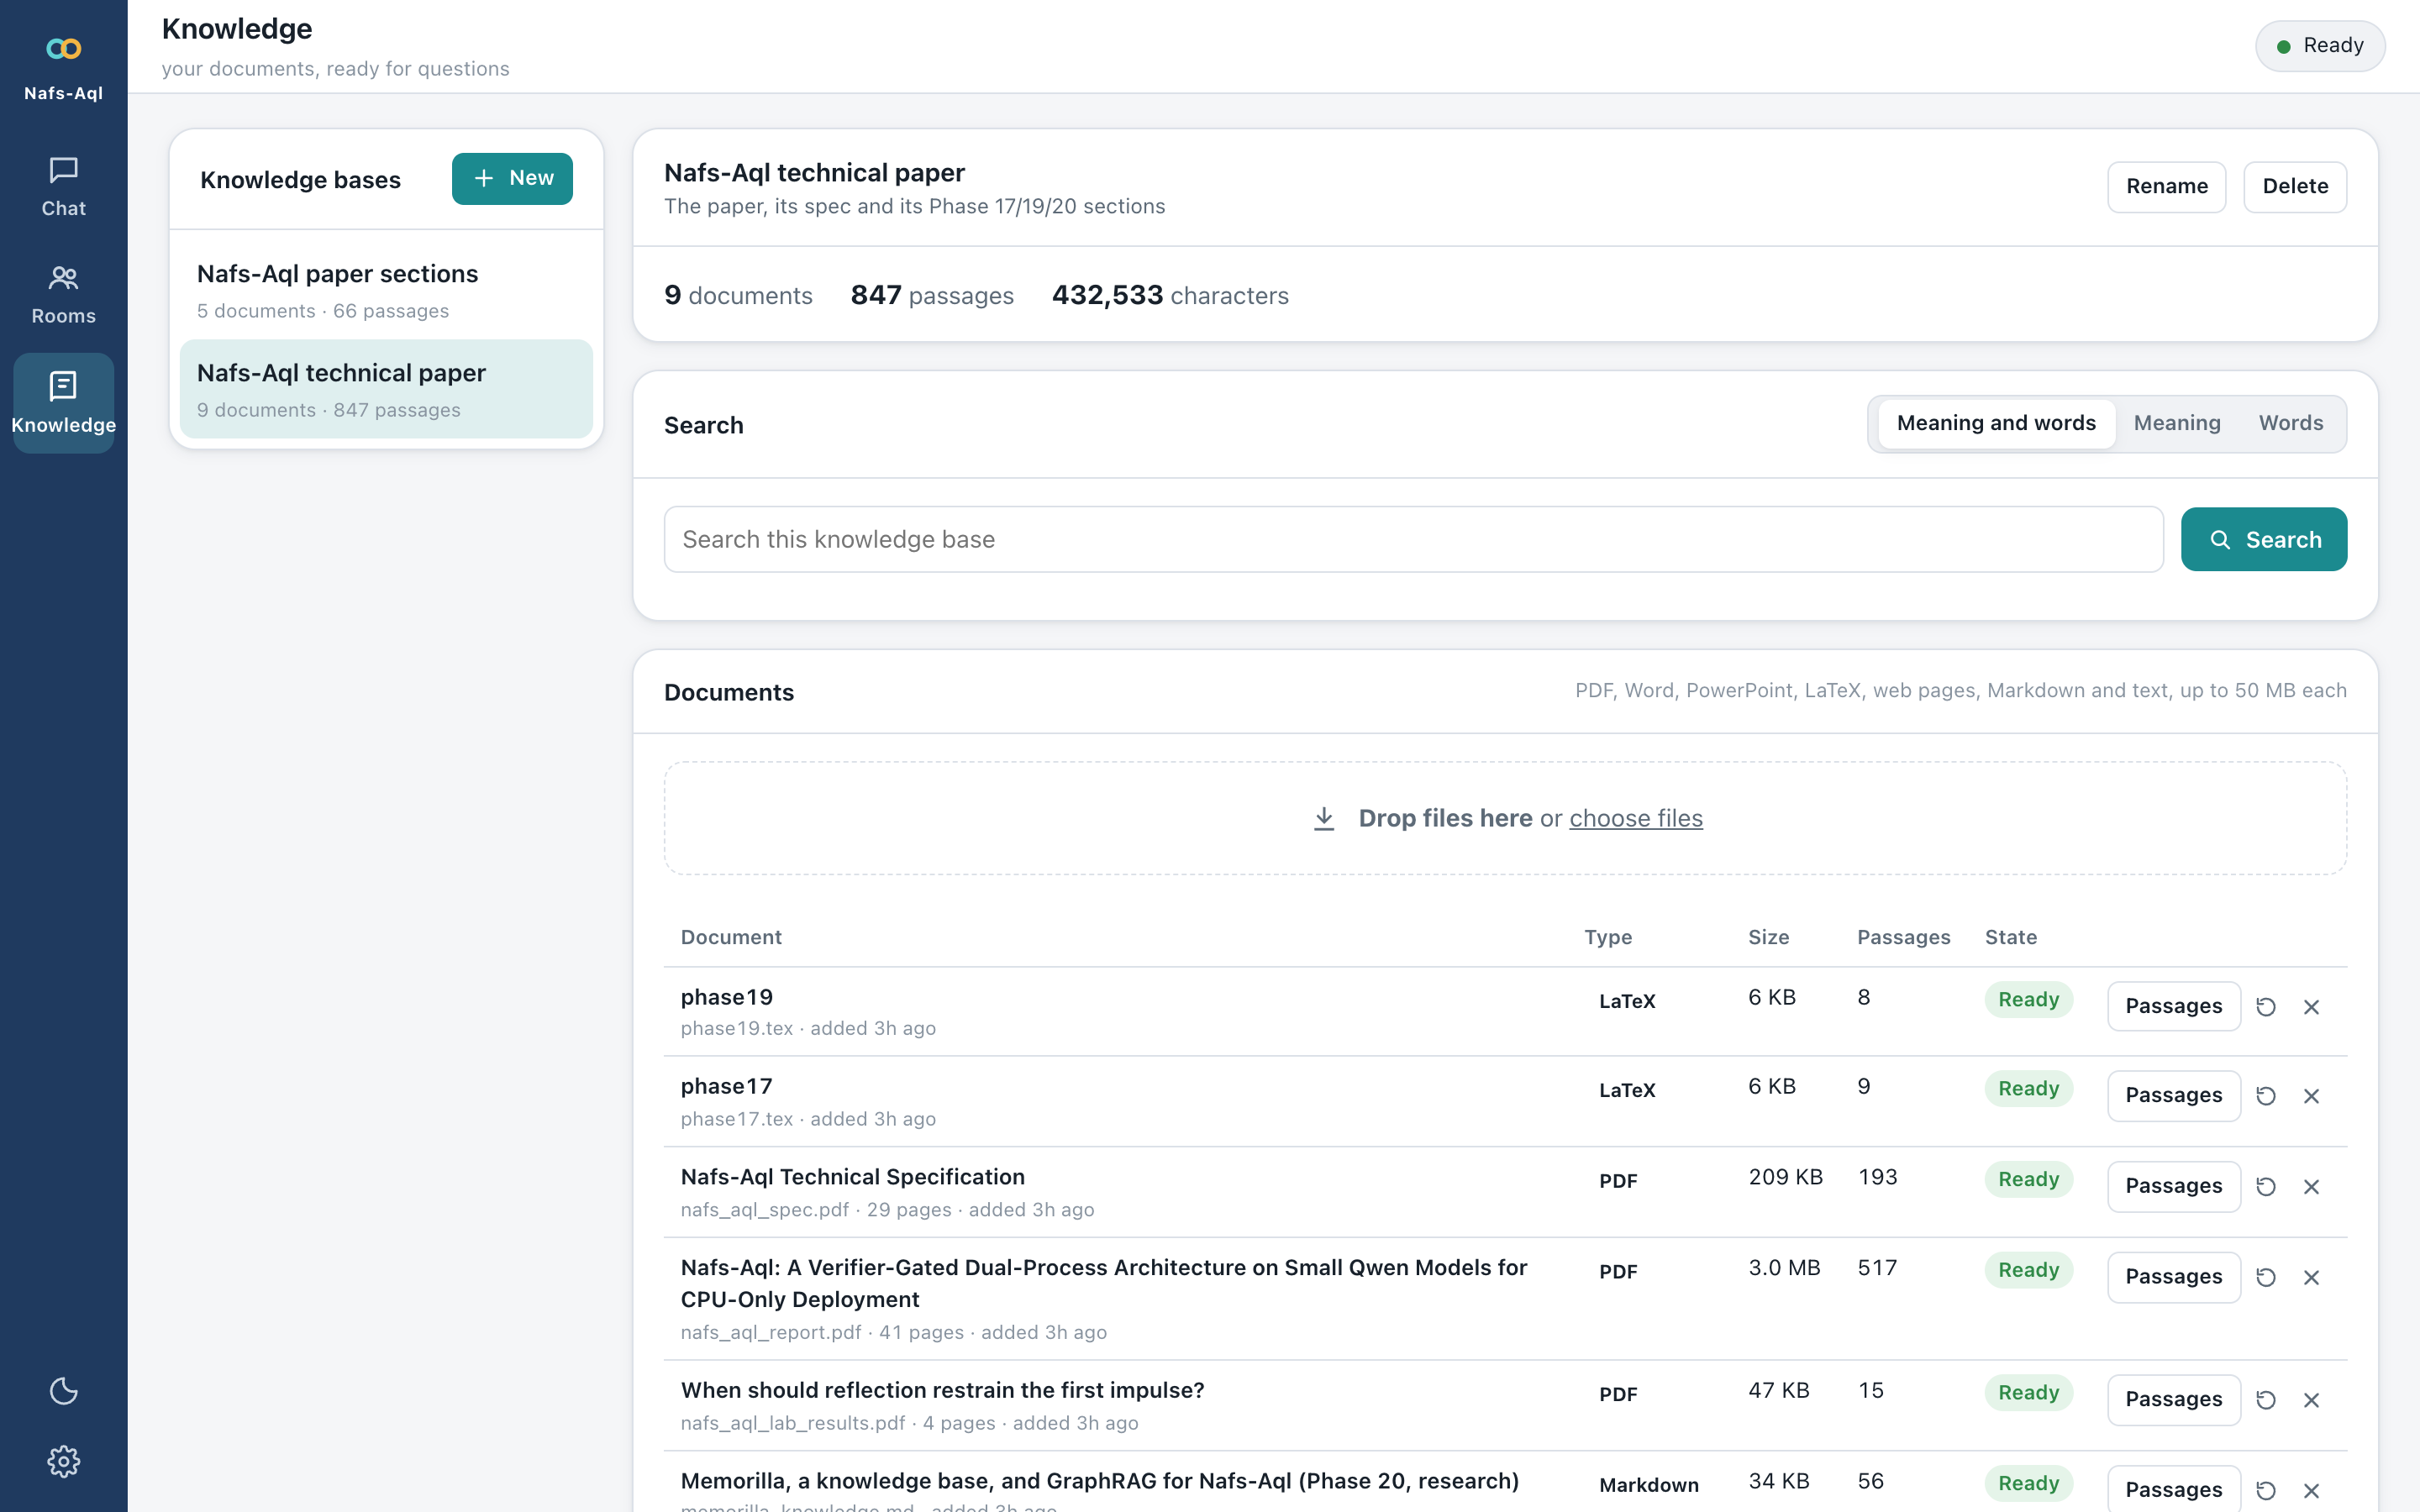
\includegraphics[width=0.48\textwidth]{../shared/screenshots/knowledge.png}\hfill
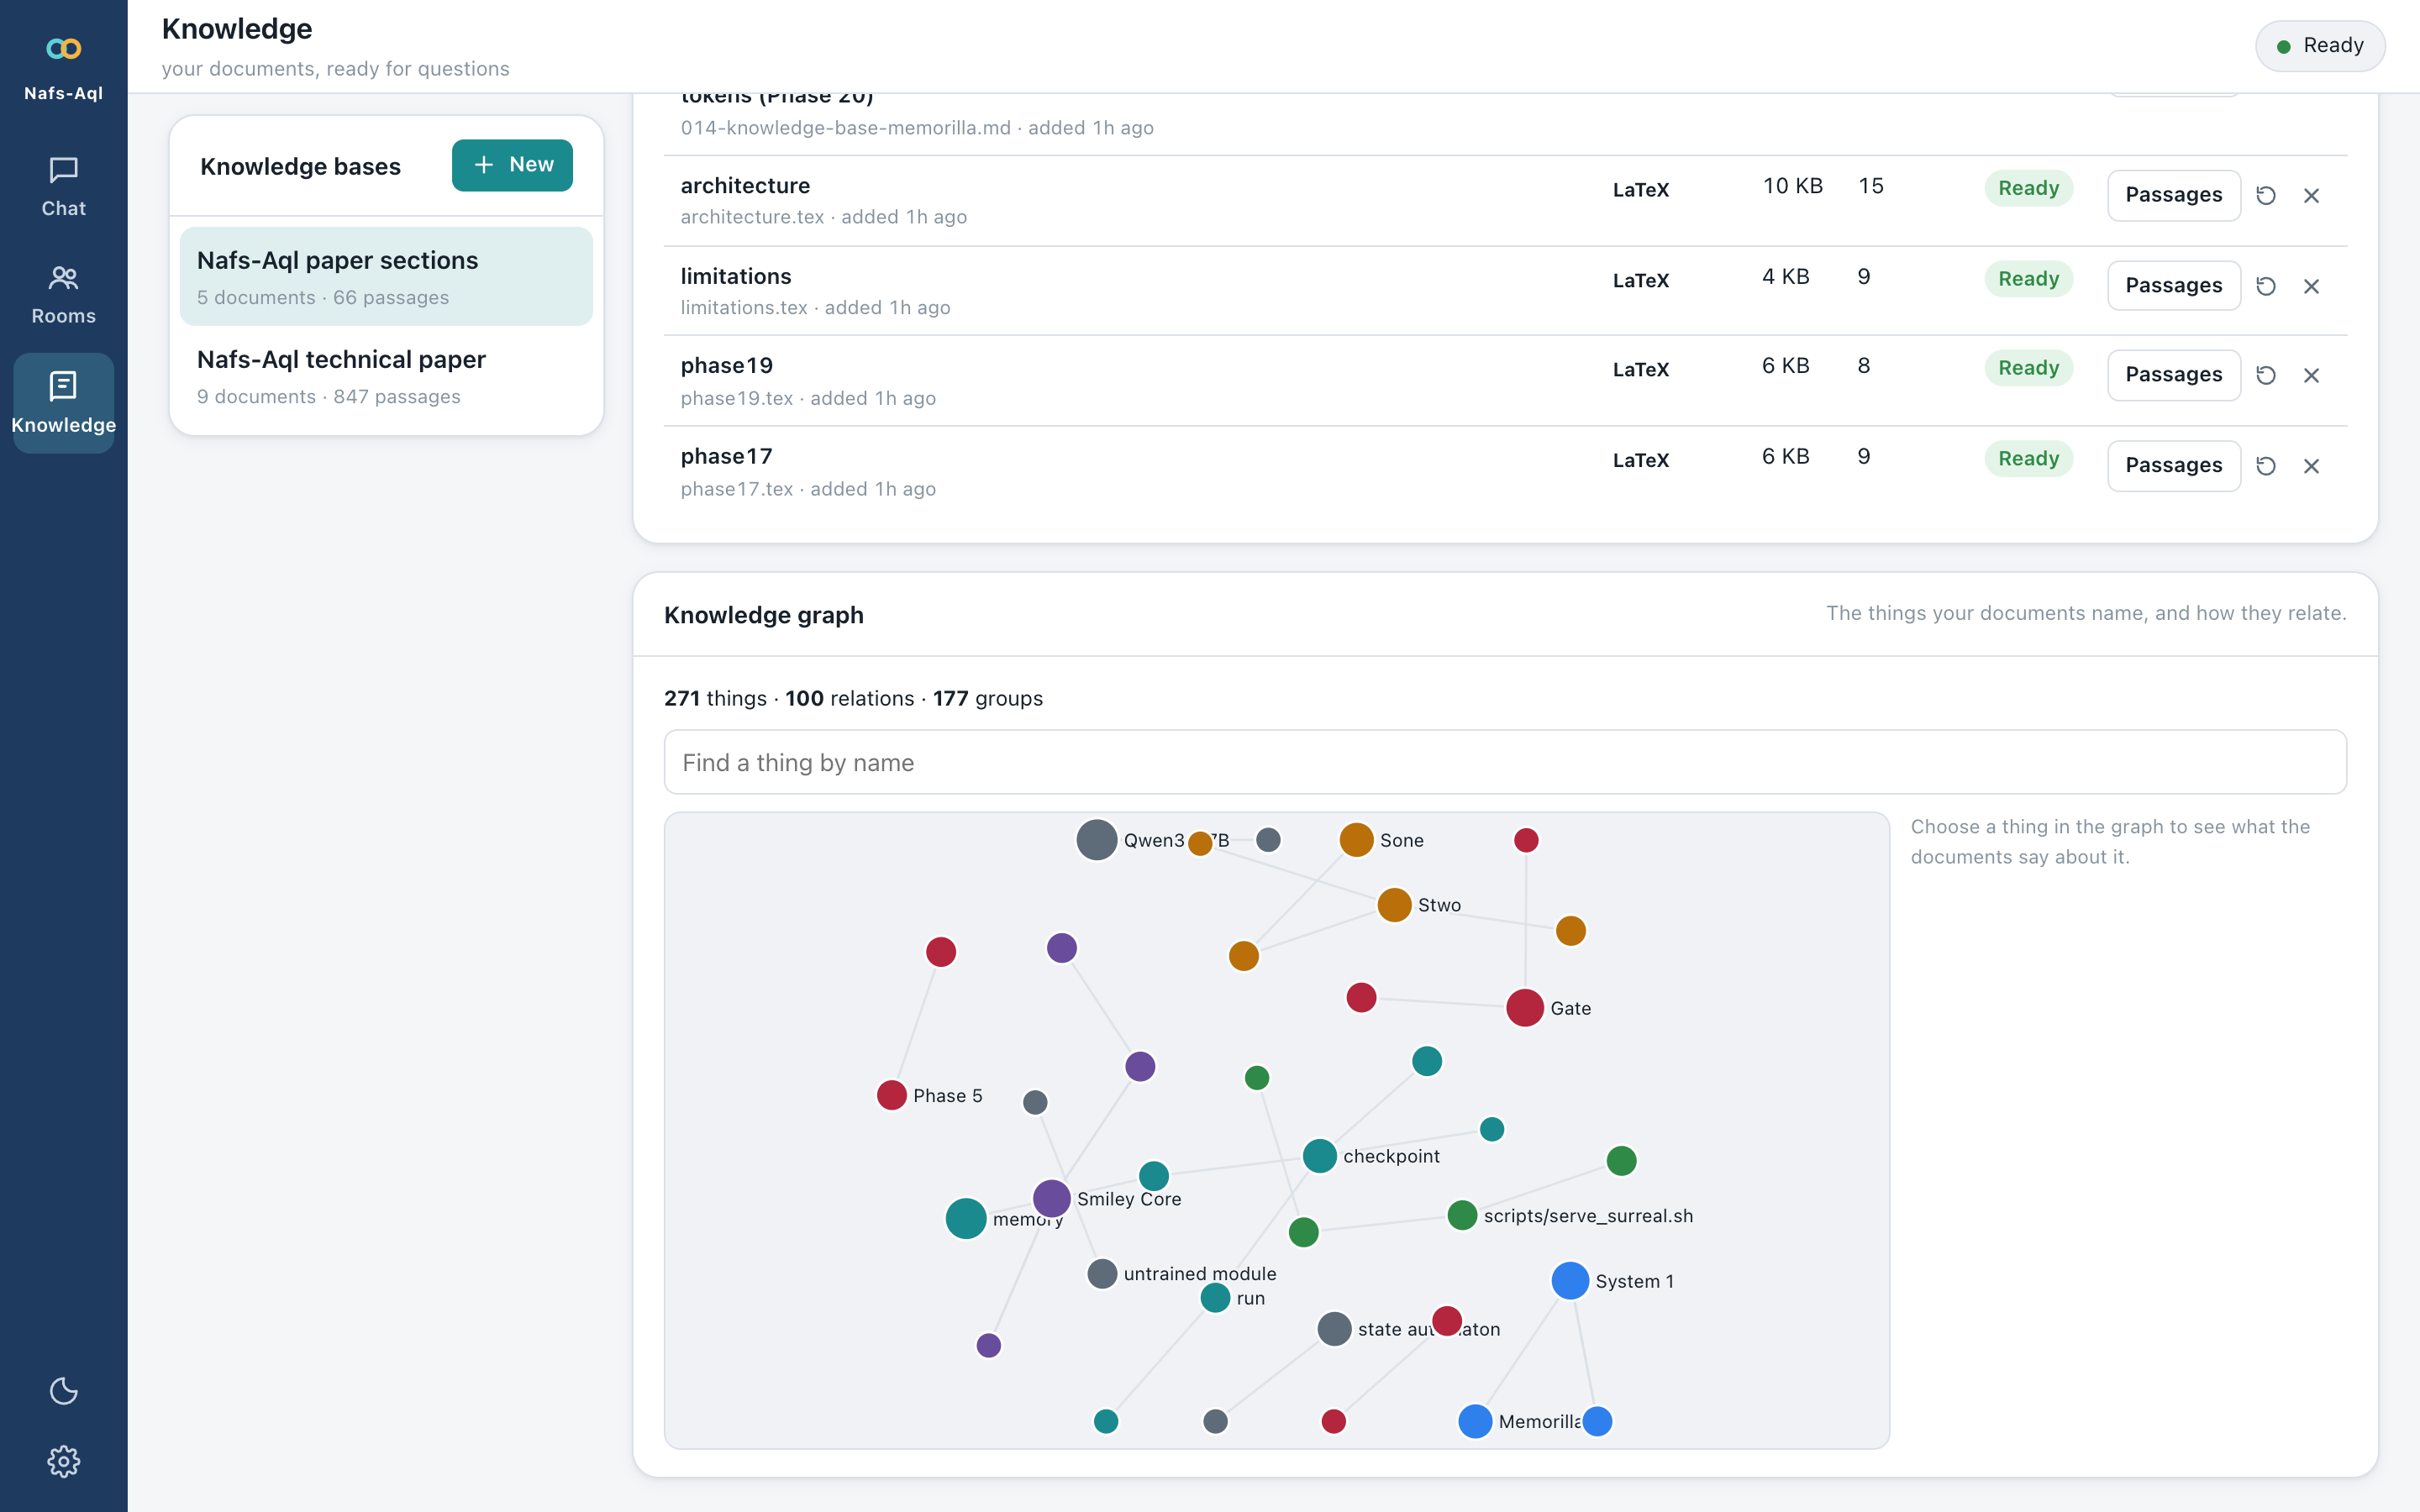
\includegraphics[width=0.48\textwidth]{../shared/screenshots/knowledge_graph.png}\\[4pt]
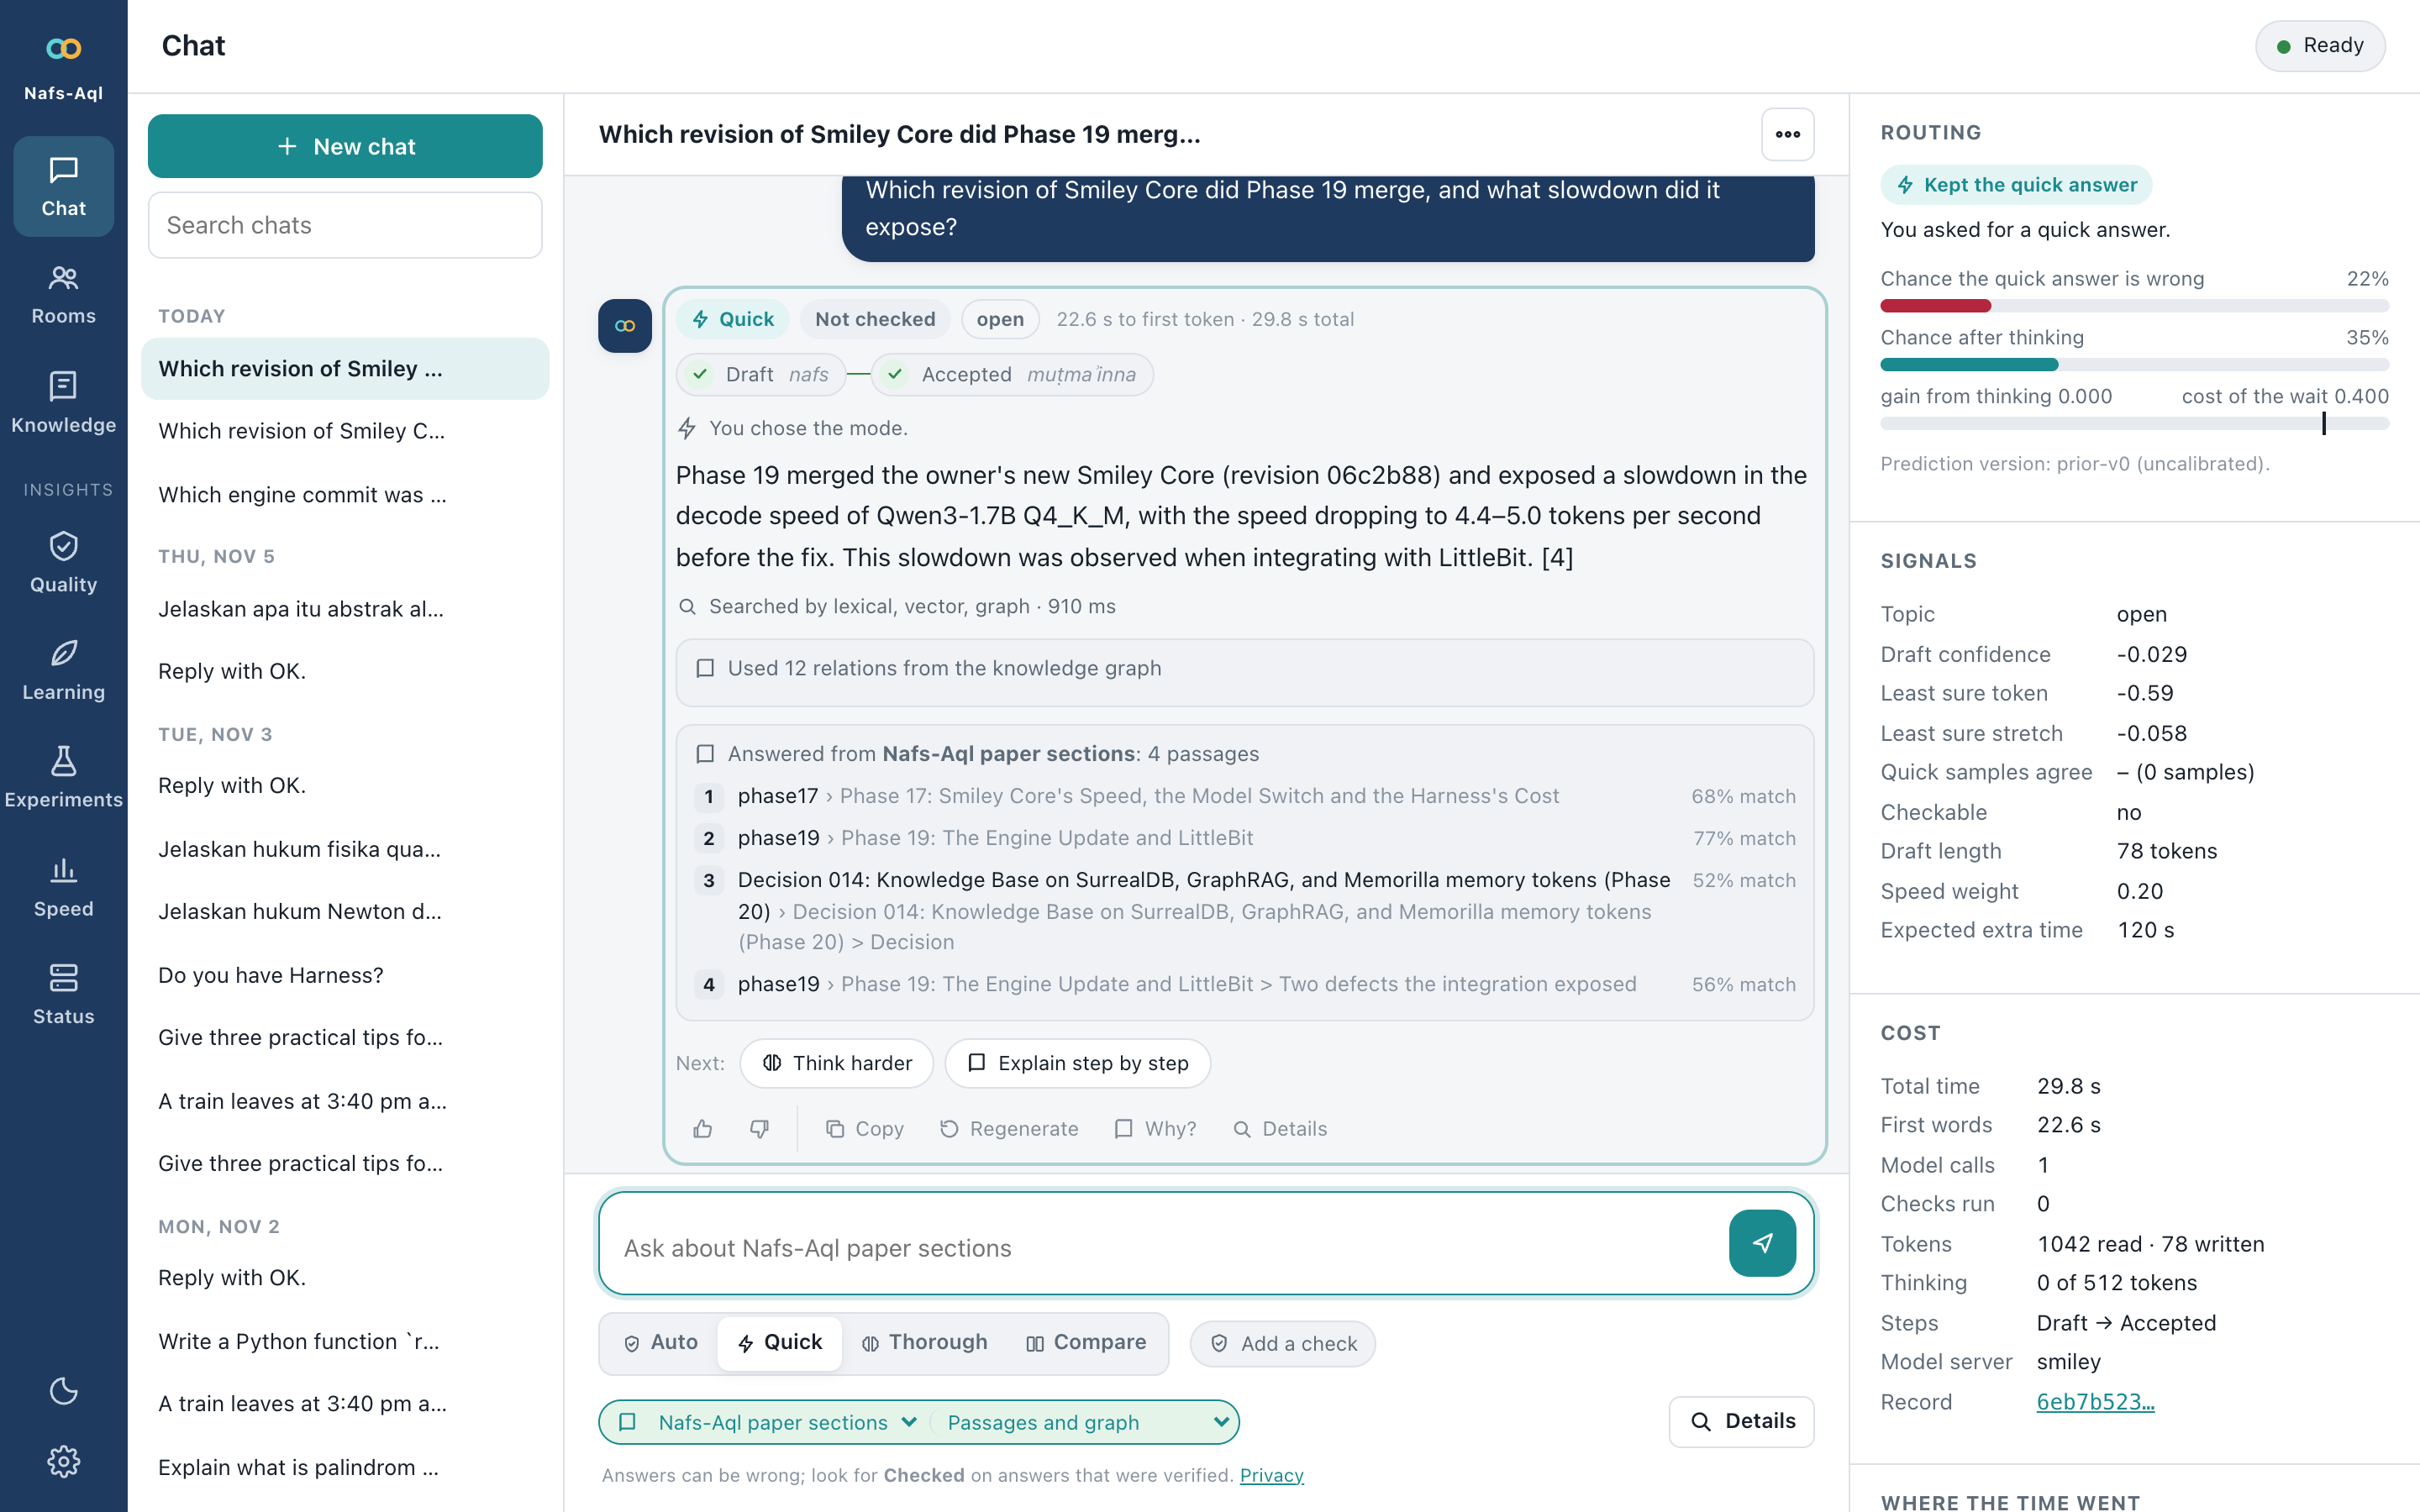
\includegraphics[width=0.9\textwidth]{../shared/screenshots/knowledge_chat.png}
\caption{The Knowledge page with the project's own paper uploaded (PDF, \LaTeX{} sections and Markdown), the graph read from it, and a chat answer
with numbered sources, the arms that ran, and a relation's verified quote.}
\label{fig:knowledge}
\end{figure}

\textbf{Ingestion.} Parsers written in Rust read PDF, Word, PowerPoint, \LaTeX{}, HTML, Markdown and text; a heading-aware chunker cuts passages of 1,200
characters with 150 of overlap, each carrying its heading path and page. Passages go into SurrealDB 3.3.5 with a BM25 full-text index and an HNSW vector index
(cosine, $M{=}12$, $\mathrm{efc}{=}150$; an exact scan below 5,000 vectors) over Qwen3-Embedding-0.6B served by Smiley Core. The client speaks CBOR because
SurrealDB's JSON decoding turns a string such as \texttt{"Caption: Model\ldots"} into a record identifier. Twenty-five papers (421 pages) parse and chunk in
32--70\,ms per page.

\textbf{Search and chat.} Words and meaning are fused by reciprocal rank~\cite{cormack2009rrf} ($k{=}60$). On twenty paraphrased questions hybrid recall@5 is
0.90, against 0.85 for words alone and 0.55 for meaning alone. Chat has six knowledge modes: \texttt{rag} (numbered passages), \texttt{graph},
\texttt{memory}, \texttt{hybrid}, \texttt{auto}, and \texttt{off}; retrieved text is delimited and labelled as data, never instructions.

\textbf{The graph.} The quick model reads each passage once under a JSON Schema and returns entities, relations, and (Phase~21) a one-line context and the
sentence that states each relation. Entities are merged by name and by the cosine of their name vectors ($\ge 0.92$), relations by their endpoints with a
weight, and Louvain communities are detected. Extraction was measured in four prompt variants on Qwen3-1.7B: objects with one worked example on an unrelated
topic gave valid, faithful JSON at 138 output tokens, against 327 for a variant with descriptions.

\textbf{Memorilla.} A 31.5\,M-parameter memory module reads the whole base once and returns sixteen vectors that replace the embeddings of sixteen
placeholder tokens in the prompt of the frozen decoder. It is implemented in Candle with parity to the unmodified PyTorch reference within
$1.9{\times}10^{-6}$ on three configurations, served through a supplied-input-vector path in Smiley Core, and trained from a knowledge base by
\texttt{memorilla-train} through a differentiable Qwen3 decoder (logits within $2{\times}10^{-5}$ of candle-transformers).

\subsection{Defects found by measuring}

\emph{Three silent gradient failures.} Candle's fused LayerNorm and \texttt{softmax\_last\_dim} have no backward pass and its autograd treats them as
constants, so only the final projection learned; \texttt{VarBuilder::get} on a \texttt{VarMap} initialises to zero; and SiLU written as
$x/(1+e^{-x})$ gives $0\cdot\infty=\mathrm{NaN}$ in the backward pass for a large negative activation. Each was found with a gradient probe and is now
covered by a test that requires a finite, non-zero gradient on every parameter.

\emph{Two read-only reviews found twelve more.} Among them: two requests could both start a trainer into one directory; activating a run that was still
training pinned a checkpoint that was then overwritten and could be read half-written (a module is now copied out on activation and saves are atomic);
a run stopped before its first step saved an untrained module as its best; a document mentioning the placeholder token in a title or heading broke memory
answers for everyone using the base; and the prepared-document cache ignored the module's weights.

\subsection{What the comparison with OntoSmith showed}

OntoSmith builds a governed graph under a human-approved, hash-pinned ontology, with a proposer that cannot write, deterministic gates, a pinned judge, and a
published record whose corrected precision is 0.911 and whose ceiling-adjusted recall is 0.203. Read against the code rather than the prose, we are already
ahead in the pieces that decide retrieval quality: it has no BM25 in its served path (a $\sum(1+\ln tf)$ stand-in), fixed 1,000-character windows without
overlap, a sentence vector index that is created and never queried, no rank fusion on its served path, and a sample API with no authentication. Three of
its claims outrun its code: its served graph carries no evidence quote, its judge never sees the ontology, and its flagship pack does not run the
configuration its record describes.

It is ahead in five things, and the gap analysis (twelve rows, nine closed in Phase~21) takes them in order of measured value. The one that matters most
explained a result of our own: our Phase~7 measurement had \texttt{graph} answering 15 of 20 questions against \texttt{rag}'s 18, winning none of the three
discordant pairs, because \texttt{graph\_search} sorted the retrieved passages by how many question entities each mentions, which pushed the passage that
holds a plain fact below passages that merely name entities. In OntoSmith the graph \emph{supplies candidates}: a triple's quote resolves to its owning chunk,
which joins the dense pool before scoring.

\subsection{What Phase 21 built}

\begin{itemize}
\item \textbf{The graph is an arm, not an override} (FR-K50). Passages cited by a fact join the candidate pool; the search's rank and the graph's rank
  (cited weight, then question entities named, over the \emph{whole} pool) are fused by reciprocal rank with a configured weight. The first test of this
  caught a flaw in the first design: ranking only the passages the graph had an opinion about let one weak mention leapfrog the search's best.
\item \textbf{Contextual BM25 and a free context line} (FR-K51, FR-K53). The words index is over the same text a passage is embedded as: title, heading
  path, context line, body, following Anthropic's contextual retrieval~\cite{anthropic2024contextual}. The context line comes out of the graph call the base
  already pays for, so it costs no extra model call. A database made before Phase~21 is migrated on first use; the live sweep found that
  \texttt{DEFINE INDEX IF NOT EXISTS} had left the old index over \texttt{text} and every lexical search failed with ``no suitable index''.
\item \textbf{A sentence packer} (FR-K52). The old block gave each passage $B/k$ characters and cut the rest, which could cut the answering sentence. The
  new block scores each sentence by its own relevance (idf-weighted overlap with the question) plus its passage's rank, both z-normalised, and fills one
  budget with whole units, skipping a unit that does not fit rather than stopping.
\item \textbf{Ontology as data and verified quotes} (FR-K54, FR-K55). The entity types and their definitions are stored with the base, served by
  \texttt{GET/PUT /v1/kb/\{kb\}/ontology}, and build the extraction prompt; a stray type is mapped onto the last declared one. A relation is stored only with
  a sentence that occurs in its passage verbatim after whitespace normalisation, and drops are counted: the gate also bounds what a document can put into a
  prompt through the graph.
\item \textbf{A two-hop walk with a path score} (FR-K56). Hop~2 keeps the best $\beta{=}8$ relations per reached entity, each scored by weight
  (normalised to the heaviest first-hop relation) times $0.6$ per hop, and a second-hop fact carries the entity it came through so the prompt shows the
  chain. This is deliberately not OntoSmith's beam, which prunes on cosine alone with no path score, no edge weight and no decay.
\item \textbf{Named arms and a failure anatomy} (FR-K59, NFR-K11). Every reply says which searches ran and why any did not. The A/B script gives each
  question exactly one fate (answered; retrieved but not used; not retrieved) and asserts that the fates sum to the set, the practice OntoSmith uses on its
  gold set.
\end{itemize}

Specified and deferred, with the reason: a reranker (needs a model download and a measured adoption; the literature's largest single jump, failure 2.9\,\% to
1.9\,\%), community summaries (one model call per community), and a confidence per relation with a review band (needs measured thresholds).

\subsection{Measurements}

\textbf{Modes, before the upgrade.} Twenty held-out questions over the fixture base, arms interleaved per question: closed-book 2/20, \texttt{rag} 18/20,
\texttt{graph} 15/20 at $1.28\times$ the time (exact McNemar $p=0.25$ against \texttt{rag}; closed-book against \texttt{rag}, $p=3.1{\times}10^{-5}$).
A defect in the grader (punctuation normalised away, so \texttt{nafs-core} could never match) moved the counts from 15/20 and 12/20 to 18/20 and 15/20 and
was found by regrading the stored answers, not by a new run.

\textbf{Memory.} The module learns from the first step (loss 8.50, 3.60, 4.08; gradient norm falling from 6,969 to about 1,200), and the untrained module reads
exactly like no module (claim accuracy 0.692 with and without it), so the path is correct. It costs 137--272\,s per example on this host against 36--94\,s
measured on a quieter one, so three epochs is 11--34 hours and the \texttt{memory} and \texttt{hybrid} arms are \emph{not measured}.

\textbf{After the upgrade, on the paper itself.} The corpus is this report and its companions: three PDFs (the report, 41 pages; the specification, 29;
the results write-up, 4), four \LaTeX{} sections and two Markdown notes, as two bases: the whole set (9 documents, 847 passages) and five sections
(66 passages) with the graph built over them (271 entities, 100 relations, 177 communities, every relation carrying a verified quote). Twenty questions
with exact expected phrases (a commit hash, a bandwidth, a version, a parameter count) were asked in each mode, arms interleaved per question
(\texttt{benchmarks/kb\_modes\_ab\_paper\_sections.json}, \texttt{kb\_modes\_ab\_paper.json}; load average 6--17). On the sections base:
closed-book 0/20, \texttt{rag} 18/20 (median 20.8\,s), \texttt{graph} 17/20 (median 25.2\,s, $1.15\times$). Against \texttt{rag}, \texttt{graph}
now loses one discordant pair and wins none (exact McNemar $p=1.0$), where before the upgrade it lost three of three; the one loss is a question that
asks which revision Phase~19 \emph{replaced}, answered with the revision it merged. On the whole-paper base: closed-book 0/20, \texttt{rag} 17/20
(median 24.2\,s, $p=1.5{\times}10^{-5}$ against closed-book). The failure anatomy names every miss: two questions were \emph{not retrieved} (a parameter
count and a cache size whose passages did not reach the prompt), one was \emph{retrieved but not used} (the quick model
answered a bandwidth question with the megabytes-per-token figure from the same passage). The ingestion of the corpus found three defects that no
fixture had: 472 of the report's 724 PDF passages carried typographic ligatures (\texttt{fi} as U+FB01) that no word search matches; \LaTeX{}
backslashes in a passage broke the extraction's JSON; and a 187-byte upload waited five minutes behind a 517-passage re-index. Each is fixed and
covered (Section~\ref{sec:phase22} for the last). The default \texttt{auto\_order} stays \texttt{["rag"]}: the graph arm no longer costs accuracy, but
on these questions it does not add any, and it costs 15\,\% of the time.

\subsection{Validation}

The workspace has 426 tests, all passing in release mode, with \texttt{rustfmt}, \texttt{clippy -D warnings} and \texttt{cargo deny} clean. A new live sweep
(\texttt{scripts/kb\_sweep.py}) covers the \texttt{/v1/kb/*} routes that no earlier suite reached: status, the life cycle of a base, ingestion end to end, the
three search modes, the graph routes, the ontology routes, the training routes, and one chat answer per mode; it passes 38 of 38 after the index migration
it found. Two CI findings are recorded rather than hidden: \texttt{cargo deny} now reports two unmaintained crates (\texttt{paste}, through candle's gemm;
\texttt{ttf-parser}, through our PDF reader, which does parse untrusted input), ignored by identifier with a written reason and a review date.
